\documentclass[a4paper,11pt,titlepage]{article}

\usepackage{latexsym}
\usepackage{graphicx}
\usepackage{float}
\usepackage{url}
\usepackage{unicode}
\usepackage[polish]{babel}
\usepackage{titlesec}
\usepackage{listings}
\usepackage{xcolor}
\usepackage{setspace}
\usepackage{subfig}
\usepackage{tabularx}
\usepackage{courier}
\DeclareUnicodeCharacter{200B}{{\hskip 0pt}}

\definecolor{codeblue}{rgb}{0,0,0.6}
\definecolor{codegray}{rgb}{0.5,0.5,0.5}
\definecolor{codepurple}{rgb}{0.58,0,0.82}
\definecolor{backcolour}{rgb}{0.96,0.96,0.96}

\lstdefinestyle{code}{
    backgroundcolor=\color{backcolour},
    keywordstyle=\color{codeblue},
    numberstyle=\tiny\color{codegray},
    stringstyle=\color{codeblue},
    basicstyle=\ttfamily\footnotesize,
    breakatwhitespace=false,
    breaklines=true,
    captionpos=b,
    keepspaces=true,
    numbers=left,
    numbersep=3pt,
    showspaces=false,
    showstringspaces=false,
    showtabs=false,
    tabsize=1,
    basicstyle=\small
}

\lstset{style=code}

\newcommand{\sectionbreak}{\clearpage}
\author{Adam Talarczyk}
\title{Symulacja Wieloagentowa}
\frenchspacing
\begin{document}
\begin{titlepage}
    \begin{center}

        \Huge
        \textbf{WYDZIAŁ NAUK ŚCISŁYCH I TECHNICZNYCH}
        
        
        \vspace{1.5cm}
	   Symulacje Komputerowe
        \LARGE
        
	\vspace{2cm}
	
	Sprawozdanie ``Symulacja Wieloagentowa''

	\vspace{1cm}
	Adam Talarczyk, Mateusz Wrzoł
	
	\vspace{5cm}
        \vfill

        \vspace{0.8cm}
	\Large
        Uniwersytet Śląski, Sosnowiec, 2021

    \end{center}
\end{titlepage}
\newpage

\tableofcontents
\newpage

\section{Zadanie 1}
Należy opracować symulator dowolnego zjawiska lub procesu, wykorzystując model wieloagentowy.

Symulator powinien być wyposażony następujące funkcje:
\begin{itemize}
\item wizualizacja stanu środowiska i agentów,
\item wykres(y) z wynikami symulacji,
\item interfejs użytkownika umożliwiający modyfikowanie parametrów modelu.
\end{itemize}


Sprawozdanie powinno zawierać:
\begin{itemize}
\item opis zaimplementowanego modelu wieloagentowego,
\item kod źródłowy symulatora z komentarzami,
\item prezentację interfejsu użytkownika z zrzutami ekranu,
\item przykładowe wyniki symulacji,
\item spis bibliografii (jeżeli była wykorzystana).
\end{itemize}

Dodatkowo poza sprawozdaniem proszę przesłać pik(i) z projektem symulatora (np. plik Netlogo).

Ocena rozwiązania będzie uwzględniała:
\begin{itemize}
\item stopień skomplikowania zaproponowanego modelu i opracowanego symulatora,
\item oryginalność rozwiązania (symulator nie może być prostą modyfikacją modeli symulacyjnych dostępnych w Netlogo lub innego gotowego oprogramowania),
\item jakość przygotowanego sprawozdania.
\end{itemize}

Do rozwiązania zadania można wykorzystać środowisko Netlogo lub dowolne inne środowisko programistyczne.

%Symulacja
\section{Symulacja środowiska ptaszników}
Wykonana w sprawozdaniu symulacja jest odwzorowaniem naturalnego środiwiska ptaszników z uwzględnieniem ich charakterystycznych zachowań. Ponadto, symulacja pozwala na zmianę wielu czynników wpływając na zachowania symulowanych obiektów.

Rozdział zawiera opis zaimplementowanego modelu wieloagentowego, kod źródłowy z komentarzami, prezentację interfejsu użytkownika oraz opis wyników symulacji.

%Opis zaimplementowanego modelu
\subsection{Opis modelu}
Stworzony model obejmuje zagadnienia związane z przebiegiem cyklu życia ptasznika, lecz bez wskazania na konkretny gatunek. Użytkownik posiada możliwość zasymulowania według własnego zamysłu grupowej hodowli ptaszników. Projekt został zaimplementowany na podstawie poniższych zagadnień: 

\begin{itemize}
  \item Ptaszniki podzielone są na dwie płcie: samiec oraz samica,  
  \item Przestrzeń, po której poruszają się ptaszniki zawiera miejsca wilgotne, a także suche, 
  \item W miejscach wilgotnych samice oraz podrostki samców zakładają gniazda, mogę jednak je opuścić w poszukiwaniu innej lokalizacji, 
  \item Na całym obszarze poruszają się owady karmowe, które służą jako pokarm dla populacji ptaszników, ich ilość jest regulowana, 
  \item Mijający czas powoduje wzrost ptaszników odpowiednio wielkościowo dla płci (pajęczaki przechodzą tak zwaną wylinkę), a także powoduje śmierć u zwierząt ze względu na podeszły wiek, 
  \item Okres oczekiwania na kolejną wylinkę ptasznika może być regulowany przez użytkownika systemu, 
  \item Spotkanie dwóch ptaszników może doprowadzić do walki pomiędzy nimi, a w następstwie śmiercią jednego z nich, 
  \item Dorosłe samce poruszają się po terytorium w poszukiwaniu samicy, w celu odbycia kopulacji, 
  \item Kopulacja może skończyć się pozytywnym scenariuszem, wtedy samica po pewnym czasie może złożyć kokon. W najgorszym wypadku samica atakuje samca i go zjada, dzieje się tak w momencie gdy samica jest głodna lub wskaźnik agresji wśród populacji znajduje się na wysokim poziomie, 
  \item Udana kopulacja nie zapewnia pewności stworzenia kokonu przez samicę, powodzenie gwarantuje odpowiedni parametr ustawiany przez użytkownika, 
  \item Dojrzałość płciową reguluje się w systemie za pomocą parametru DC, w żargonie terrarystyki jest to długość ciała zwierzęcia,  
  \item Złożenie kokonu odbiera samicy połowę maksymalnej energii, a opieka nad kokonem samica sprawuje do czasu jego otwarcia, 
  \item Inkubacja kokonu trwa przez okres zdefiniowany przez użytkownika, 
  \item Z otwierającego się kokonu wychodzi określona przez użytkownika ilość nimf (okres życia ptasznika po wylęgu), 
  \item Warunki atmosferyczne (temperatura i wilgotność) mają wpływ na życie ptaszników oraz szansę otwarcia się kokonu, niekorzystne warunki powodują wymieranie populacji, 
Wskaźniki numeryczne oraz wykresy wskazują parametry związane z ilością poszczególnych elementów w symulacji oraz ich zmiany w przeciągu interwałów czasowych. 
\end{itemize}

%Sources
\subsection{Kod źródłowy symulatora- wybrane fragmenty}
W tym rozdziale zostaną zaprezentowane kluczowe elementy kodu źródłowego symulacji. Podstawowym elementem symulacji są agenci, których implementacja jest zawarta w listingu \ref{lst:1}. 

\begin{lstlisting}[language=HTML, caption=Implementacja agenta w środowisku NetLogo, label={lst:1}]
breed [spiders spider]
spiders-own [ sex dc energy nest health last-molt]
\end{lstlisting}

\noindent W linii pierwszej definiuje się agenta typu “spiders”, zaś linia druga określa parametry z nim związane.  

W sekcji “setup” ustawiane są wartości związane z podstawowymi parametrami symulacji, szczegóły zostały zaprezentowane w listingu \ref{lst:2}. 

\begin{lstlisting}[language=HTML, caption=Ustalanie podstawowych parametrów symulacji. , label={lst:2}]
to setup
  clear-all
  reset-ticks
  set-default-shape spiders "spider"
  set-default-shape bugs "bug"
  set-default-shape cocoons "egg"
  set maxsize-female 1.1
  set maxsize-male 0.95
  set-background
  spawn-spiders
end
\end{lstlisting}

\noindent W linii 2 oraz 3 usuwane są wartości pochodzące z poprzedniego użycia symulacji, następnie (linia 4, 5, 6, 7 i 8) zostają ustalone kształty jakie zostają nadane poszczególnym agentom oraz nadania im maksymalnego rozmiaru. Stworzenie tła na podstawie zdefiniowanej procedury znajduje się w linii 9, zaś pojawienie się ptaszników uzależnione jest od wywołania w linii 10. 

Zdefiniowanie podstawowych zmiennych związanych z ptasznikiem zawarte jest w listingu \ref{lst:3}, także tutaj znajduje się w linii 1 stworzenie według parametru, określonej liczby ptaszników: 

\begin{lstlisting}[language=HTML, caption=Metoda odpowiadająca za tworzenie obiektu typu ``ptasznik samica''., label={lst:3}]
create-spiders ilosc_samic [
    set color pink
    setxy random-xcor random-ycor
    set energy 100
    set health 100
    set sex 1
    set nest false
    set dc max_dc
    set last-molt ticks
    set size maxsize-female
  ]
\end{lstlisting}

Wykonywanie się poszczególnych funkcji jest uzależnione od zawarcia jej w sekcji “go”. W tym miejscy wykonuje się dla każdego z agentów określona procedura, która musi zostać do niego przypisana. W listingu \ref{lst:4} został pokazany przykład na podstawie symulacji.

\begin{lstlisting}[language=HTML, caption= Sekcja ``go'' symulacji., label={lst:4}]
to go
  if not any? spiders [ stop ]
  spawn-food
  ask spiders
  [ move
    eat
    will-fight
    reproduce
    make-nest
    molting
    male-wait-to-grow-up
    random-disaster
    death ]

  ask bugs
  [ move-food
    death-food ]

  ask cocoons
  [ hatch-cocoon ]
  tick
end
\end{lstlisting}

\noindent Sekcja “go” (linia od 1 do 20) wykonuje się w momencie istnienia przynajmniej jednego ptasznika, potwierdza to kod znajdujący się w linii 2. W danym ticku (jednostka miary symulacji) wykonuje się dla obiektów symulacji szereg procedur (na podstawie ptasznika od linii 4 do 13), następnie proces przechodzi do kolejnego ticku (linia 19) i tym samym się zapętla przechodząc ponownie do linii 1.  

Zachowanie agenta jest uzależnione od zaimplementowanej funkcji wywoływanej w procedurze “go”. Przykładowa zawartość takiego elementu znajduje się w listingu \ref{lst:5}.

\begin{lstlisting}[language=HTML, caption= Przykładowa procedura ``reproduce'', label={lst:5}]
to reproduce
  let candidate one-of spiders-at 1 0
  if candidate != nobody [
    if (([sex] of candidate) = 1 and sex = 0 and
      ([nest] of candidate) = true) [
      if ([energy] of candidate < 50)[
        set health 0
        ask candidate [ set energy 100 ]
      ]
      if([dc] of candidate) >= dc_kopulacja and dc >= dc_kopulacja and health != 0[
        create-cocoon
      ]
    ]
  ]
end
\end{lstlisting}

\noindent Linia 2 ładuje do zmiennej “candidate“ informacje na temat napotkanego agenta tego samego typu- spiders. W momencie gdy obiekt nie jest pusty (linia 3), sprawdza się warunek, czy dany ptasznik jest samcem a spotkany obiekt samicą, ulokowaną w swoim gnieździe (linia 4 i 5). Wartość “true” obliguje do weryfikacji parametru odpowiadającego za energię samicy, wartość mniejsza od 50 powoduje, że samiec zostaje zjedzony przez samicę, zyskując maksymalną ilość energii. W przeciwnym wypadku porównywana jest minimalna wielkość ptasznika zdolnego do kopulacji. Spełnienie warunku wywołuje procedurę “create-cocon”, odpowiedzialną za utworzenie kokonu przez samicę (linia 11). 

%Interfejs
\subsection{Interfejs użytkownika}
Interfejs użytkownika został przedstawiony na rysunku \ref{fig:9}, wyszczególnić można 3 kategorie:
\begin{itemize}
	\item Konfiguracja symulacji i środowiska
	\item Pole na którym wyświetlana jest symulacja
	\item Panel raportowania, zawierający dane i wykresy
\end{itemize}

\begin{figure}[H]
\centering
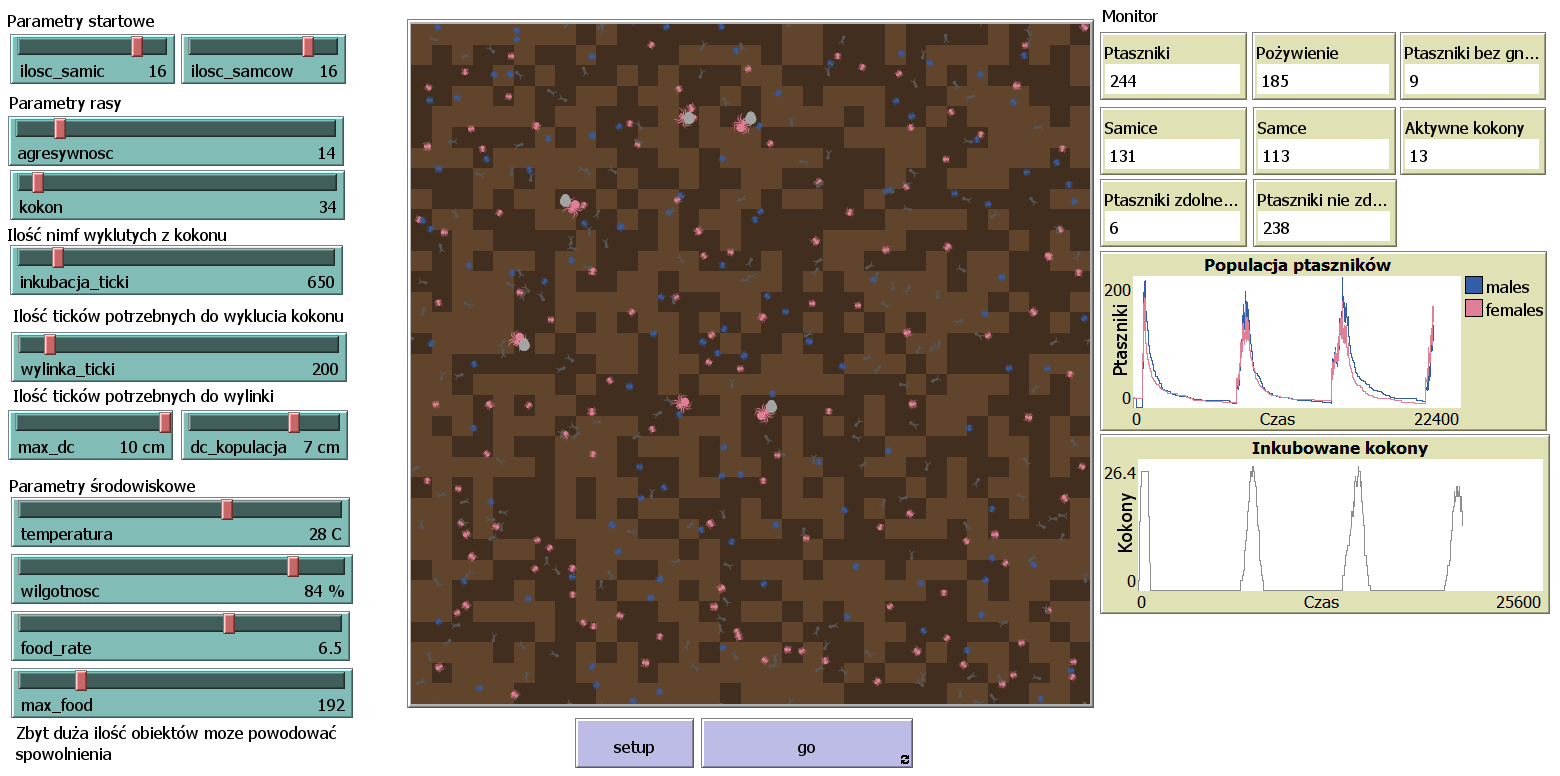
\includegraphics[width=1\columnwidth]{img/symulacja.PNG}
\caption{Obszar symulacji}
\label{fig:9}
\end{figure}

% Opis parametrów i kontrolek
Obszar konfiguracji środowiska również podzielony jest na kategorie. Parametry startowe zaprezentowane na rysunku \ref{fig:6} (tj. \textit{ilosc\_samic}, \textit{ilosc\_samcow}) określają ile dorosłych samic i samców podczas inicjalizacji ma zostać wygenerowanych.

\begin{figure}[H]
\centering
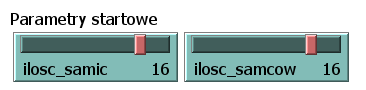
\includegraphics[width=.5\columnwidth]{img/parametry_startowe.PNG}
\caption{Kontrolki odpowiedzialne za parametry startowe}
\label{fig:6}
\end{figure}

Parametry rasy (rysunek \ref{fig:5} określają ogólne zachowanie ptaszników:
\begin{itemize}
\item \textit{agresywnosc} - zachowanie w stosunku do innych ptaszników. Wartość 0 oznacza, że nie będąze sobą w ogóle walczyć, \item wartość 100 – walka przy każdym spotkaniu. 
\item \textit{kokon} - ilość młodych nimf wyklutych z pojedynczego kokonu 
\item \textit{inkubacja\_ticki} - ilość czasu potrzebne do wyinkubowania kokonu
\item \textit{wylinka\_ticki} - ilość czasu, potrzebna do odbycia kolejnej wylinki. Wylinka wiąże się ze wzrostem DC pająka. 
\item \textit{max\_dc} – maksymalny rozmiar, który może osiągnąć ptasznik. 
\item \textit{dc\_kopulacja} – wymagany rozmiar ptasznika aby osiągnąć zdolności kopulacyjne 
\end{itemize}

\begin{figure}[H]
\centering
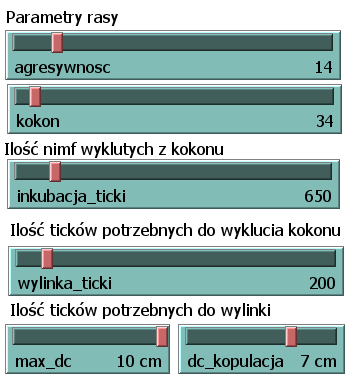
\includegraphics[width=.5\columnwidth]{img/parametry_rasy.PNG}
\caption{Kontrolki odpowiedzialne za parametry rasy}
\label{fig:5}
\end{figure}


Parametry środowiskowe - ogólne parametry odpowiedzialne za środowisko, temperaturę, wilgotność oraz ilość pożywienia na ekranie (rysunek \ref{fig:4}):
\begin{itemize}
\item \textit{temperatura}, \textit{wilgotnosc} - parametry, które mogą być zmieniane podczas symulacji. Stosując wartości skrajne można spowodować zachowania uboczne, np. Umieranie ptaszników, niszczenie kokonów.
\item \textit{food\_rate} - mnożnik jedzenia, im większy, tym więcej pożywienia pojawia się na ekranie.
\item \textit{max\_food} - maksymalna ilość pożywienia na ekranie jednocześnie. Zbyt duża ilość może powodować problemy optymalizacyjne. 
\end{itemize}

\begin{figure}[H]
\centering
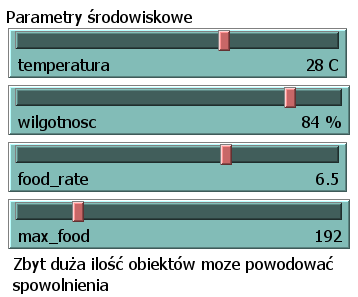
\includegraphics[width=.5\columnwidth]{img/parametry_env.PNG}
\caption{Kontrolki odpowiedzialne za parametry środowiskowe}
\label{fig:4}
\end{figure}

% opis symulacji i ikon
Obszar symulacji zaprezentowano na rysunku \ref{fig:1}. Po obszarze poruszają się ptaszniki, których płeć można rozróżnić przez charakterystyczne kolory. Kolor różowy oznacza samicę, a niebieski samca (rysunek \ref{fig:icons1}). Dodatkowo, na obszarze symulacji wyszczególnić można ikony kokonu i pożywienia (rysunek \ref{fig:icons2}).
\begin{figure}[H]
\centering
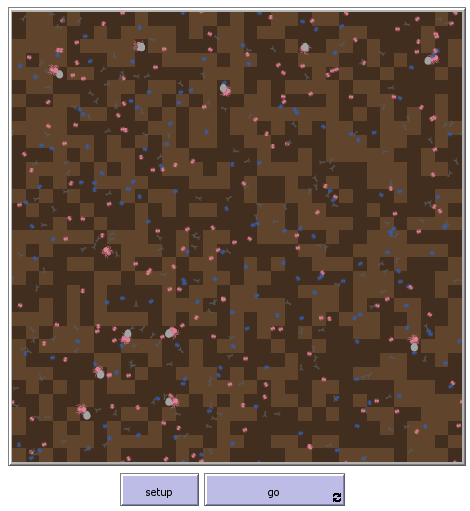
\includegraphics[width=.75\columnwidth]{img/map.PNG}
\caption{Obszar wizualizacji symulacji}
\label{fig:1}
\end{figure}

\begin{figure}[H]%
    \centering
    \subfloat[\centering Ikona samicy]{{
\includegraphics[width=3cm]{img/samica.PNG} }}%
    \qquad
    \subfloat[\centering Ikona samca]{{
\includegraphics[width=3cm]{img/samiec.PNG} }}%
    \caption{Ikony samców i samic w symulacji}%
    \label{fig:icons1}%
\end{figure}

\begin{figure}[H]%
    \centering
    \subfloat[\centering Ikona pokarmu]{{
\includegraphics[width=3cm]{img/bug.PNG} }}%
    \qquad
    \subfloat[\centering Ikona kokonu]{{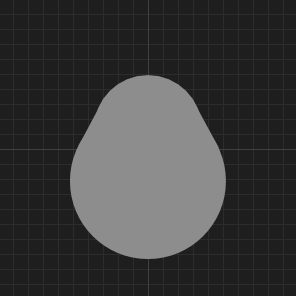
\includegraphics[width=3cm]{img/egg.PNG} }}%
    \caption{Pozostałe ikony użyte w symulacji}%
    \label{fig:icons2}%
\end{figure}

Dodatkowo, środowisko NetLogo pozwala na śledzenie obiektów w czasie rzeczywistym, zaprezentowane zostało to na rysunku \ref{fig:8}

\begin{figure}[H]
\centering
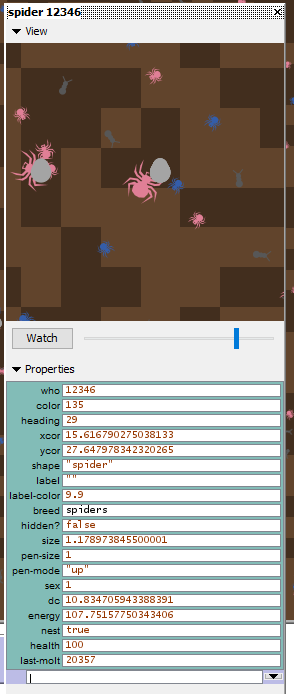
\includegraphics[width=.5\columnwidth]{img/spider-params.PNG}
\caption{Parametry ptasznika w trakcie trwania symulacji.}
\label{fig:8}
\end{figure}


%Opis danych i wykresów
Ostatnim elementem jest prezentacja danych i wyników. Odpowiedzialne jest za to monitor (rysunek \ref{fig:2}). 
\begin{figure}[H]
\centering
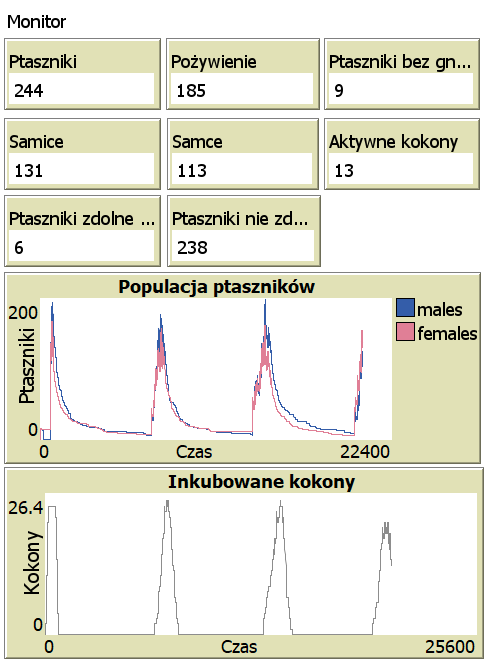
\includegraphics[width=.5\columnwidth]{img/monitor.PNG}
\caption{Monitor - reprezentacja danych symulacji}
\label{fig:2}
\end{figure}

\noindent Monitor podzielony został on na dane i wykresy. Dane przedstawiają sumaryczna ilość ptaszników z podziałem na samce, samice, ptaszniki zdolne i niezdolne do kopulacji. Dodatkowo, wyświetlana jest ilość pożywienia, ilość ptaszników bez gniazda oraz aktywne, inkubowane kokony (rysunek \ref{fig:3}).

\begin{figure}[H]
\centering
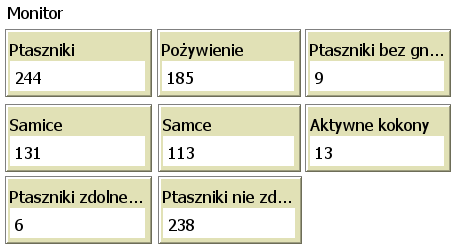
\includegraphics[width=.5\columnwidth]{img/monitor_danych.PNG}
\caption{Poszczególne dane}
\label{fig:3}
\end{figure}

Wykresy przedstawiają w czasie rzeczywistym populację ptaszników z podziałem na samce i samice. Ostatni wykres przedstawia ilość kokonów (rysunek \ref{fig:10}).
\begin{figure}[H]
\centering
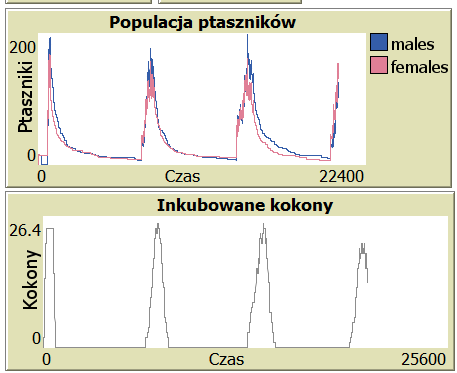
\includegraphics[width=.8\columnwidth]{img/wykresy.PNG}
\caption{Wykresy}
\label{fig:10}
\end{figure}

\subsection{Wyniki symulacji}
Wyniki symulacji przedstawiane są w czesie rzeczywistym na monitorze danych. Wizualna reprezentacja przedstawiona jest na wykresach (rysunek \ref{fig:10}). Zauważyć można zależność, że populacja ptaszników rośnie i maleje co jakiś interwał. Wynika to z charakterystyki ich zachowania, samce żyją znacznie krócej od samic i umierają niedługo po wylince umożliwiającej im kopulację. Ilość ptaszników, które przeżywa zależna jest od ilości pożywienia, agresywności rasy i innych przypadkowych czynników. Podsumowując, tylko niewielka ilość ptaszników dożywa momentu, w którym jest zdolna do kopulacji. Mimo to, w symulacji występuje ciągłość- gatunek nie wymiera przy optymalnych parametrach.

\subsection{Kod źródłowy- pełny}
\begin{lstlisting}[language=HTML, caption=Pełny kod źródłowy, label={lst:full}]
breed [spiders spider]
spiders-own [ sex dc energy nest health last-molt]

breed [bugs bug]
bugs-own [ energy-value energy ]

breed [cocoons cocoon]
cocoons-own [ tick-created ]

globals [ maxsize-female maxsize-male ]

;;Setup i inicjalizacja
to setup
  clear-all
  reset-ticks
  set-default-shape spiders "spider"
  set-default-shape bugs "bug"
  set-default-shape cocoons "egg"
  set maxsize-female 1.1
  set maxsize-male 0.95
  set-background
  spawn-spiders
end

to set-background
  ask patches [
    if random-float 1000 < 500 [ set pcolor 31 ]
    ifelse random-float 1000 > 500 [ set pcolor 32 ]
    [ set pcolor 33 ]
  ]
end

to spawn-spiders
  create-spiders ilosc_samic [
    set color pink
    setxy random-xcor random-ycor
    set energy 100
    set health 100
    set sex 1
    set nest false
    set dc max_dc
    set last-molt ticks
    set size maxsize-female
  ]
  create-spiders ilosc_samcow [
    set color blue
    setxy random-xcor random-ycor
    set energy 100
    set health 100
    set sex 0
    set nest false
    set dc max_dc
    set last-molt ticks
    set size maxsize-male
  ]
end


;;Ptaszniki - zachowanie
to go
  if not any? spiders [ stop ]
  spawn-food
  ask spiders
  [ move
    eat
    will-fight
    reproduce
    make-nest
    molting
    male-wait-to-grow-up
    random-disaster
    death ]

  ask bugs
  [ move-food
    death-food ]

  ask cocoons
  [ hatch-cocoon ]
  tick
end

to move
  ifelse nest [
    set energy energy - 0.1
  ][
    rt random 50
    lt random 50
    fd 1
    set energy energy - 0.5
  ]
end

;Walka
to will-fight
  let candidate one-of spiders-at 1 0
  if candidate != nobody [
    if random 100 < agresywnosc [
      ifelse([dc] of candidate) <= dc_kopulacja and dc <= dc_kopulacja[
        fight
      ][
        if([sex] of candidate) = sex [ fight ]
      ]
    ]
  ]
end

to fight
  let candidate one-of spiders-at 1 0
  if candidate != nobody [
    ifelse([dc] of candidate) > dc [
      set health 0
    ]
    [
      ask candidate [ set health 0 ]
    ]
  ]
end

to eat
  let candidate one-of bugs-at 1 0
  if candidate != nobody [
    if(energy < 100) [set energy energy + ([energy-value] of candidate)]
  ]
end

to reproduce
  let candidate one-of spiders-at 1 0
  if candidate != nobody [
    if (([sex] of candidate) = 1 and sex = 0 and
      ([nest] of candidate) = true) [
      if ([energy] of candidate < 50)[
        set health 0
        ask candidate [ set energy 100 ]
      ]
      if([dc] of candidate) >= dc_kopulacja and dc >= dc_kopulacja and health != 0[
        create-cocoon
      ]
    ]
  ]
end

to create-cocoon
  let candidate one-of spiders-at 1 0
  hatch-cocoons 1 [
    set color 6
    set size 1
    set tick-created ticks
    setxy [pxcor] of candidate [pycor] of candidate
  ]
  ask candidate [ set energy energy / 1.5]
end

to hatch-cocoon
  ask cocoons [
    if ticks > tick-created + inkubacja_ticki [
      ifelse( temperatura > 20 and wilgotnosc > 50) [
        hatch-spiders kokon [
          setxy random-xcor random-ycor
          set energy 30
          set health 100
          set sex random 2
          ifelse sex = 1 [set color pink][set color blue]
          set nest false
          set dc 1
          set size 0.5
          set last-molt ticks
        ]
      ][die]

      die
    ]
  ]
end

to molting
  ask spiders [
    if ticks > last-molt + wylinka_ticki [
      set last-molt ticks

      ifelse(sex = 0)[
        ;male
        ifelse(dc < max_dc) [set dc dc * 1.07][die]
        if(size < maxsize-male) [set size size * 1.07]
      ][
        ;female
        if(dc < max_dc) [set dc dc * 1.1]
        if(size < maxsize-female) [set size size * 1.1]
      ]
      if( random 10000 > 9980 ) [die]

    ]
  ]
end

to death
  if energy < 0 [ die ]
  if health <= 0 [ die ]
end

to make-nest
  if (pcolor = 32 and sex = 1 and random 1000 > 900) [
    set nest true
  ]
end

to random-disaster
  let candidate one-of cocoons-at 0 0
  if (random 1000 > 995 and sex = 1 and candidate = nobody) [set nest false]
  if (random 1000 > 995 and sex = 0) [set nest false]
end


to male-wait-to-grow-up
  if (sex = 0) [
    ifelse dc < dc_kopulacja [
      set nest true
    ][
      set nest false
    ]
  ]
end

;;Pozywienie - zachowanie
to spawn-food
  if random-float 10 < food_rate [
    if count bugs < max_food [
      create-bugs 1 [
        set color 3
        set size 0.5
        set energy-value random 20
        set energy random 50
        setxy random-xcor random-ycor
      ]
    ]
  ]
end

to move-food
  rt random 50
  lt random 50
  fd 1
  set energy energy - 0.1
end

to death-food
  if energy < 0 [ die ]
end

;;Dane i statystyki
to-report count-males
  let counter 0
  ask spiders [
    if sex = 0 [set counter counter + 1]
  ]
  report counter
end

to-report count-females
  let counter 0
  ask spiders [
    if sex = 1 [set counter counter + 1]
  ]
  report counter
end

to-report count-can-copulate
  let counter 0
  ask spiders [
    if (dc >= dc_kopulacja) [set counter counter + 1]
  ]
  report counter
end

to-report count-cannot-copulate
  let counter 0
  ask spiders [
    if (dc < dc_kopulacja) [set counter counter + 1]
  ]
  report counter
end

to-report count-spiders-without-nest
  let counter 0
  ask spiders [
    if (nest = false) [set counter counter + 1]
  ]
  report counter
end
\end{lstlisting}

\newpage
\addcontentsline{toc}{section}{Spis rysunków}
\listoffigures
\newpage

\addcontentsline{toc}{section}{Listingi}
\lstlistoflistings

\begin{thebibliography}{5}
\addcontentsline{toc}{section}{Bibliografia}
\bibitem{1}
https://ccl.northwestern.edu/netlogo/docs/programming.html
\bibitem{2}
https://ccl.northwestern.edu/netlogo/docs/dictionary.html

\end{thebibliography}


\end{document}
